Deep Neural Networks (DNNs) are an extremely successful tool, they are widely
adopted commercially and closely studied academically, however even given the
attention they have gathered there is no comprehensive understanding of how
these models generalize data and provide such impressive performance - in fact
very little is know about how DNNs learn or about their inner workings. Recently
Prof.\ Tishby produced a paper claiming to understand the basic principle of how
DNNs work. He suggested that there are two phases that the network goes trough
while being trained - the fitting phase and the compression phase. During the
fitting phase the network memorizes the training data and makes predictions
based on what it has seen before, during the compression phase the network
generalizes, it forgets the unnecessary information from the training data.
Tishby suggested that the incredible performance that DNNs are able to achieve
is due to this compression phase, and that this process of compression is a
result of randomness inherent in Stochastic gradient descent. Tishby showed this
by looking at DNNs trough the information domain, most notably he used what is
now called the information plane. The information plane summarizes how the
information is flowing trough the DNN, for every neuron layer the plane shows
mutual information it has with the input data and the label data. In his
experiments Tishby has concluded that every layer loses unnecessary information
from the input data and tries to keep information of the label.
Tishby made some interesting and significant claims about how DNNs work, however
he did no provide a formal proof, his conclusion are based only on experimental
evidence. 

In our work we look at Tishby's claim that DNNs compress data and throw away
unnecessary information about the input. We reimplement his experiments as a
form of independent verification, showing that the results Tishby got are robust
and are stable to parameter changes. We also take a look at a paper produced by
Saxe that provides an opposing view to that of Tishby's. Saxe showed that
compression that Tishby showed is only a result of Tishby's choice of
activation function for the neural network. He showed that compression only
happens when Tanh activation function is used and does not happen when ReLu is
used.

Lastly, we think that the experiments presented in both papers don't fully align
with the ideas that Tishby presented to us, specifically his idea that weights
should be treated "as if" they are random variables. Tishby's and Saxe's
experiment deal with this "as if" random notion quite crudely or try to sidestep
it completely. As a result we devised an experiment that tries to capture this
idea more explicitly, although it is still relatively crude and more work should
be put into it in the future.

\section{The Information plane}

If we look at a neural network trough the lens of information we can think of it
as a form of a Markov chain. Where every node takes in a piece of data processes
it and passes to the next node. For every such node $ t \in T $ we can measure
it's mutual information with the input patterns $ x \in X $ and labels $ y \in Y
$. 

$$ Y - X \rightarrow T_1 \rightarrow ... \rightarrow T_i \rightarrow \hat{Y} $$

In this analogy a node corresponds to a layer in a non-convolutional neural
network. When looking at a neural network in this way we can say that it's job
is to preserve as much information as possible about the label, or to minimise
information loss about the label during the transitions from node to node.

The Information plane summarized this Markov chain view and applies it to the
entirety of the training process.

\begin{figure}[H]
  \centering
  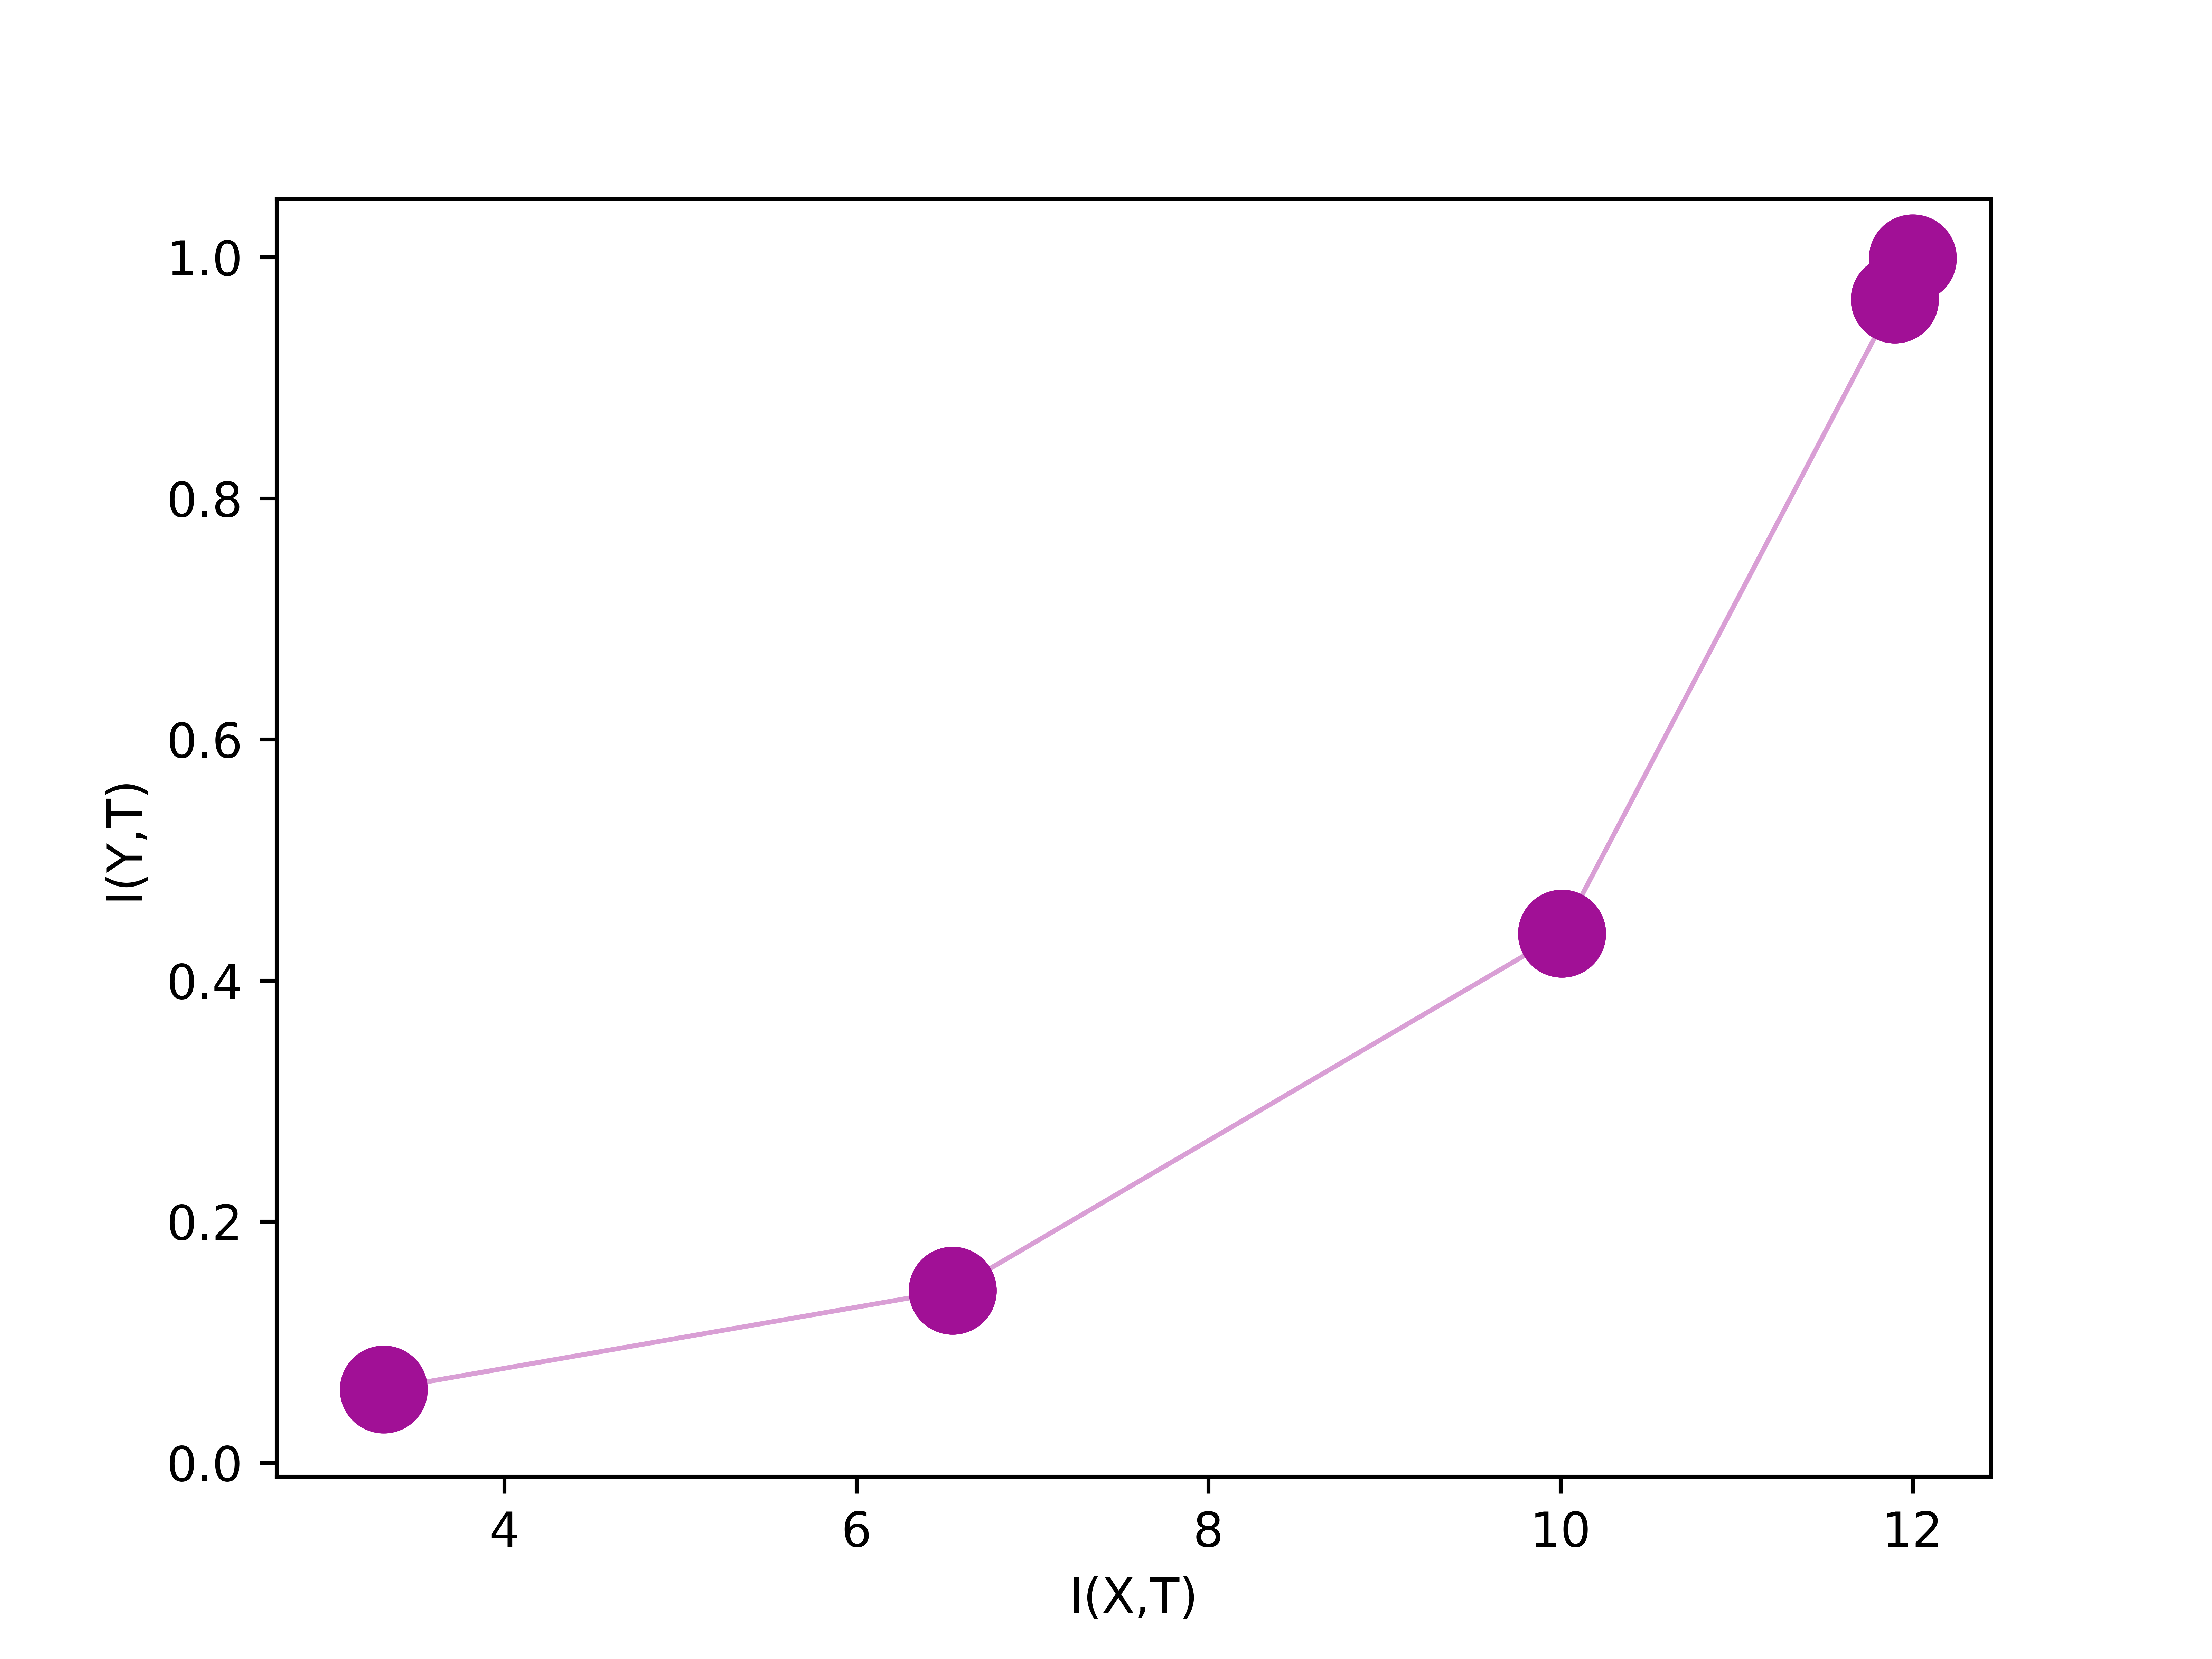
\includegraphics[width=0.65\textwidth]{figs/ip_1v2.png}
  \caption{
    information plane for a neural network with 5 layers, which was only trained
    for one epoch.
  }
  \label{fig:ip1}
\end{figure}

\autoref{fig:ip1} shows an example of an information plane - in this case the
network has 5 layers and has only been trained for one epoch. Every node
corresponds to a layer, and the lines between them just help us distinguish the
order of the layers. The $ x-axis $ shows mutual information between any layer $
T $ and the input $ X $, while the $ y-axis $ shows mutual information with the
label $ Y $.

The figure bellow corresponds to a network that takes in a 12bit number and maps
it to a 1bit number hence the mutual information ranges from 0 to 12 for the $
x-axis $ and from 0 to 1 for the $ y-axis $.

The upper right most node corresponds with the very first layer before any data
processing occurs, therefore it has maximum mutual information with the input
and the label. As the network was only trained for one epoch the weight are
essentially random and we see a steep drop in every subsequent layer, with the
last layer of the network having close to 0 mutual information with $ X $ and $
Y $, which is what we expect if we assume that the network guesses at random
before any training is done.

\begin{figure}[H]
  \centering
  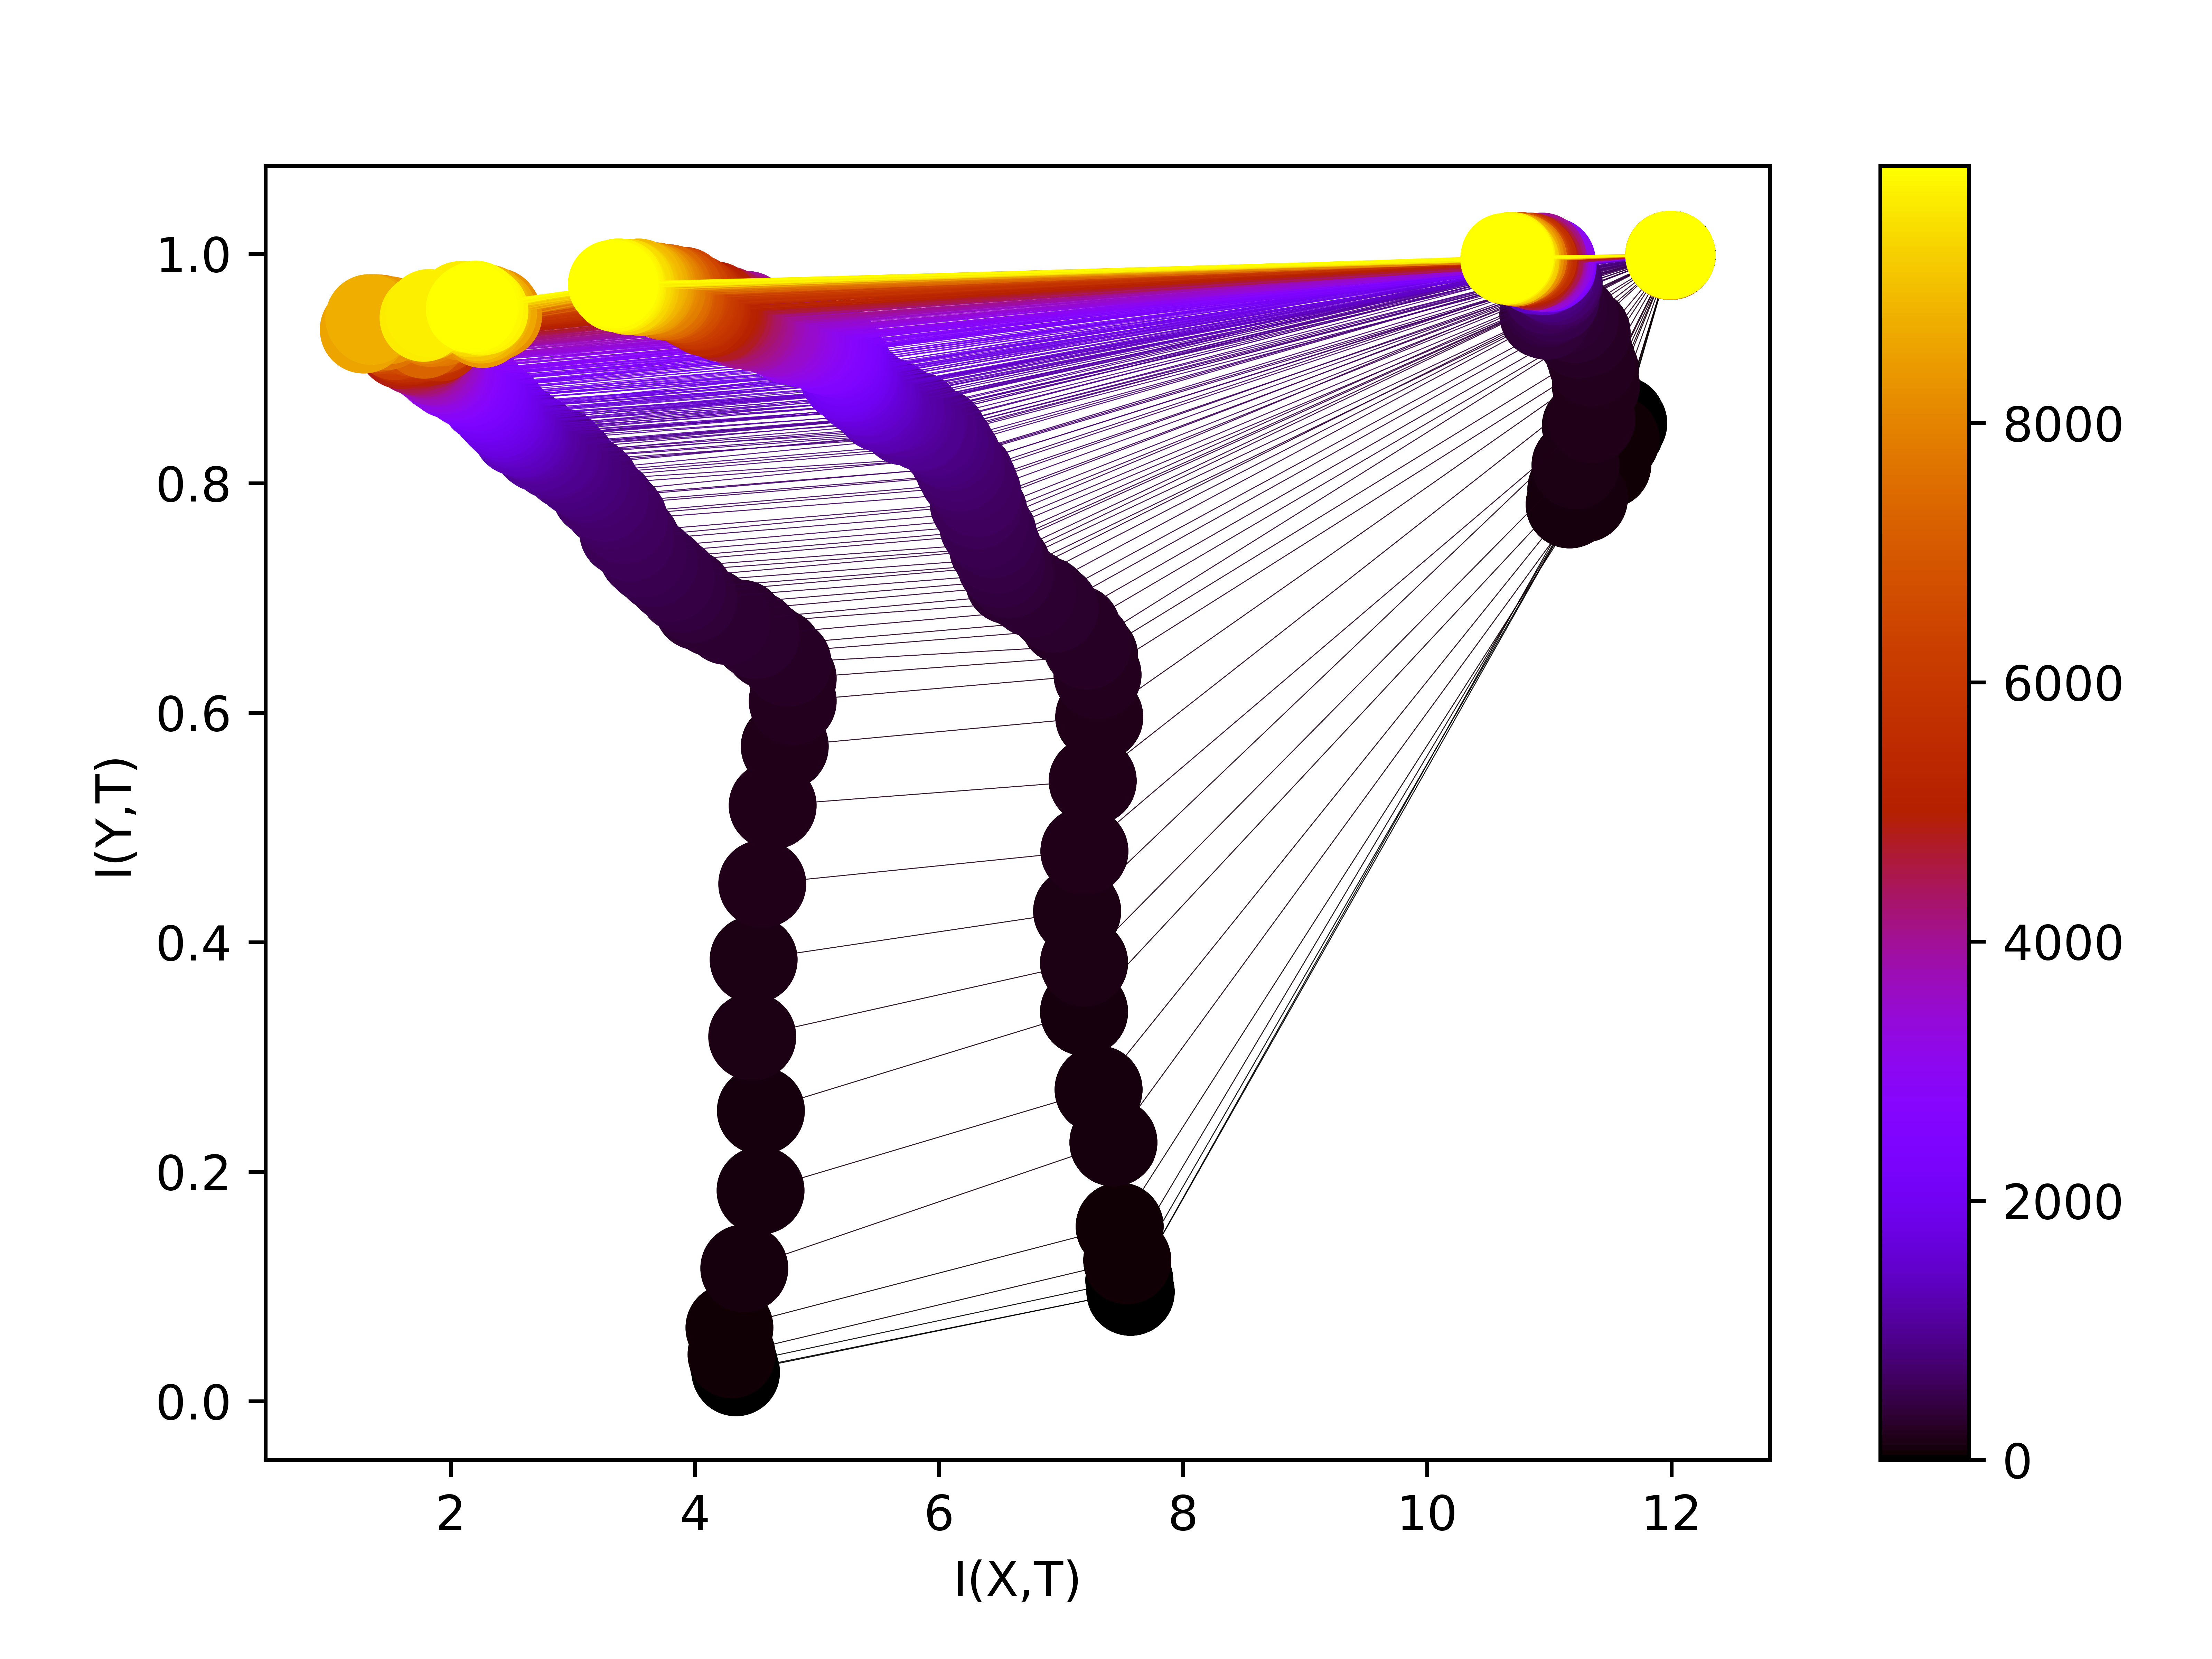
\includegraphics[width=0.65\textwidth]{figs/ip_10000.png}
  \captionof{figure}{
    Information plane for a neural network with 4 layers, which was trained for
    approximately $ 10\,000 $ epochs
  }
  \label{fig:ip2}
\end{figure}

\autoref{fig:ip2} shows an example of a full information plane. The gradient
maps the colour to the epoch. From this figure we can clearly see the fitting
and the compression phases Tishby was describing. 

\begin{itemize}
  \item{
      The Fitting phase is the rapid improvement phase at the start of the
      training period, where information about the label is rapidly increasing
      while information about the input remains approximately the same. In this
      case the training is in the fitting phase for less than 1000 epochs.
    }
  \item{
      The Compression phase begins when the after the fitting phase ends and the
      rapid improvement stops. We can see during this phase we start losing
      information about the input while still gaining information about the
      label. This phase the was majority of the training time.
    }
\end{itemize}
